\section{Flavor Tagged Jets} \label{sec:objects:flavor_tagging}

In general our reconstruction algorithms for jets are agnostic to the ``flavor"
label - light ($l$), charm ($c$), or bottom ($b$) - of the hadrons produced in
the shower.  However, flavor tagging is a powerful tool for discriminating the
$b\bar{b}$ decay products of the Higgs from the large, predominantly
light-flavor, multijet background \cite{Aad:2015ydr}.  These $b$-quark
initiated jets are identified using the \texttt{MV2c10}
\cite{ATL-PHYS-PUB-2015-022} Boosted Decision Tree (BDT) \footnote{The name
\texttt{MV2c10} means that this multivariate algorithm had a training sample
with roughly $\sim10\%$ $c$-jets and $\sim90\%$ $l$-jets in order to define a
good balance of $c$-jet and $l$-jet rejection.}, trained with a machine learning
algorithm that uses the weighted score from a series of decision trees to give
a discriminant for how similar any given jet is to a $b$-jet.  The BDT uses
inputs from the kinematics of the jet ($\pT$ and $|\eta|$) and the
outputs of tracking algorithms, discussed below, to look for signatures
consistent with a $b$-hadron decay as shown in \Cref{sec:objects:b_decay}.
Tracking information is crucial to flavor tagging, and thus the flavor tagging can only be applied
within the tracking volume ($|\eta| < 2.5$).

\begin{figure}[!htbp]
  \centering
  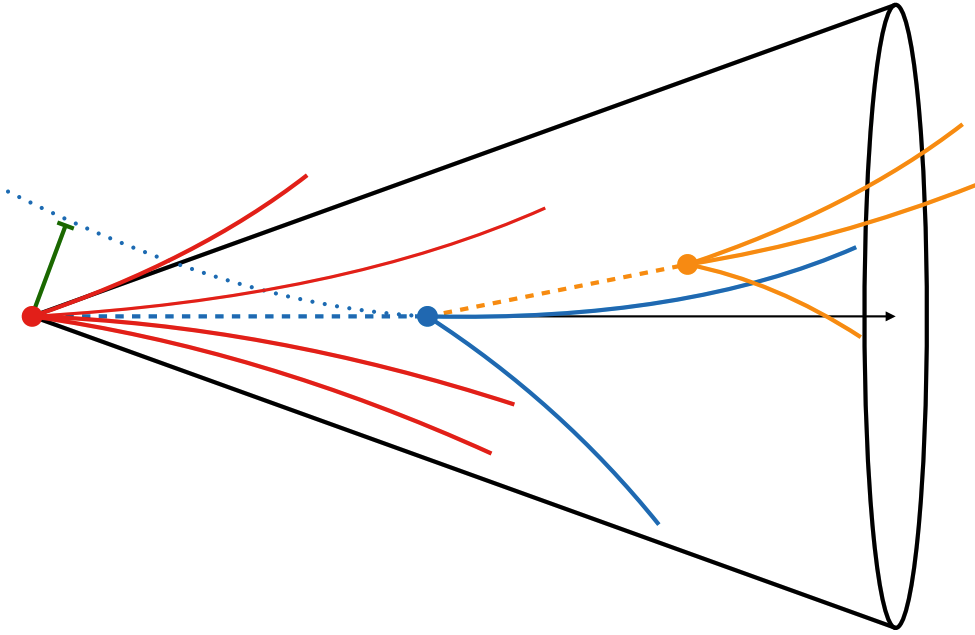
\includegraphics[width=0.8\linewidth]{figures/objects/b_decay}
  \caption{Cartoon of a $b$-jet decay containing a $b$-hadron decay vertex
(\textcolor{track_blue}{blue}~\protect\tikzdot{track_blue}) displaced from the
primary $pp$ vertex (\textcolor{red}{red}~\protect\tikzdot{red}), and a
$c$-hadron decay vertex (\textcolor{orange}{orange}~\protect\tikzdot{orange})
further displaced and often close to the $b$-hadron flight axis
\cite{Chisholm:bjet}. The secondary (\textcolor{track_blue}{blue}) and tertiary
(\textcolor{orange}{orange}) vertices have large impact parameters
(\textcolor{IPgreen}{green}) with respect to the primary $pp$ vertex.}
  \label{sec:objects:b_decay}
\end{figure}

The relatively long lifetime of $b$-hadrons ($\approx 1.5~\ps$) gives them a
characteristic length scale of  $c\tau \sim .45~\mm$. This means the $b$-hadron
travels the non-negligible distance of $\sim 5~\mm$  from the primary
interaction vertex before decaying assuming $\gamma = 10$.  This macroscopic
flight distance is large enough that this decay can be identified as a
secondary vertex (SV) displaced from the original primary vertex (PV).
Furthermore, roughly 90\% of $b$-jets will contain a $c$-jet which will create
a tertiary vertex when it decays (TV) \cite{Chisholm:bjet}.  The secondary
vertex finding algorithm (SV1), and Kalman filter algorithm (JetFitter) look
for events matching this characteristic $b$-hadron decay chain. 

Using tracking information the two-dimensional and three-dimensional impact
parameter algorithms, IP2D and IP3D, determine the transverse and longitudinal
impact-parameters - $d_{\text{0}}$ and $z_{\text{0}}$ - respectively. Looking
at \Cref{sec:objects:impact_parameters} the impact parameters of
the $b$-flavor jets tend to be positive while those of $c$-jets and $l$-jets
tend to be distributed more symmetrically around 0.

\begin{figure}[!htbp]
  \centering
  \subcaptionbox{Transverse Impact Parameter $d_{0}$}{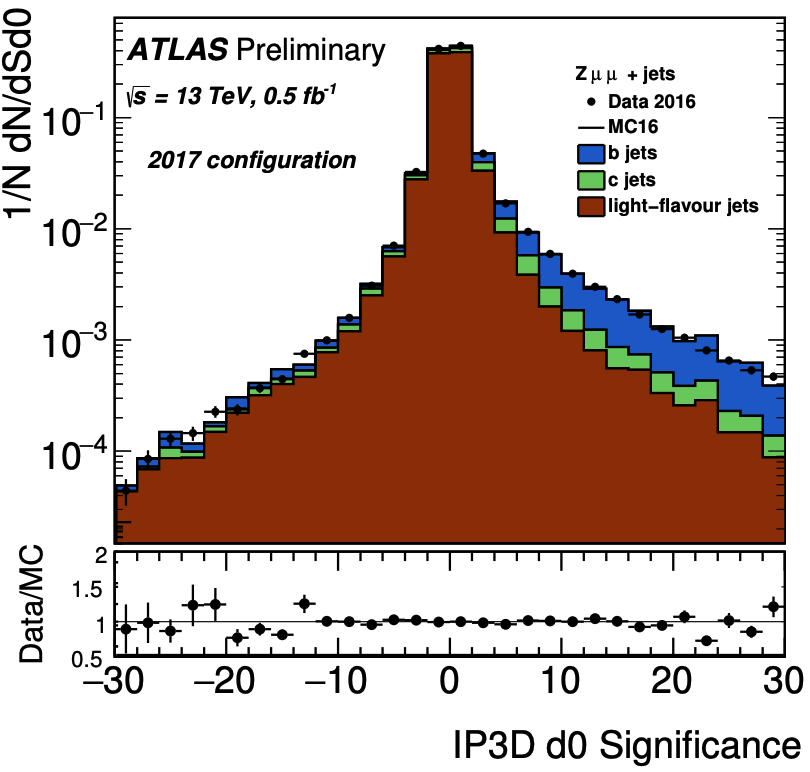
\includegraphics[width=0.48\linewidth]{figures/objects/IP3D_d0}} \hfill
  \subcaptionbox{Longitudinal Impact Parameter $z_{0}$}{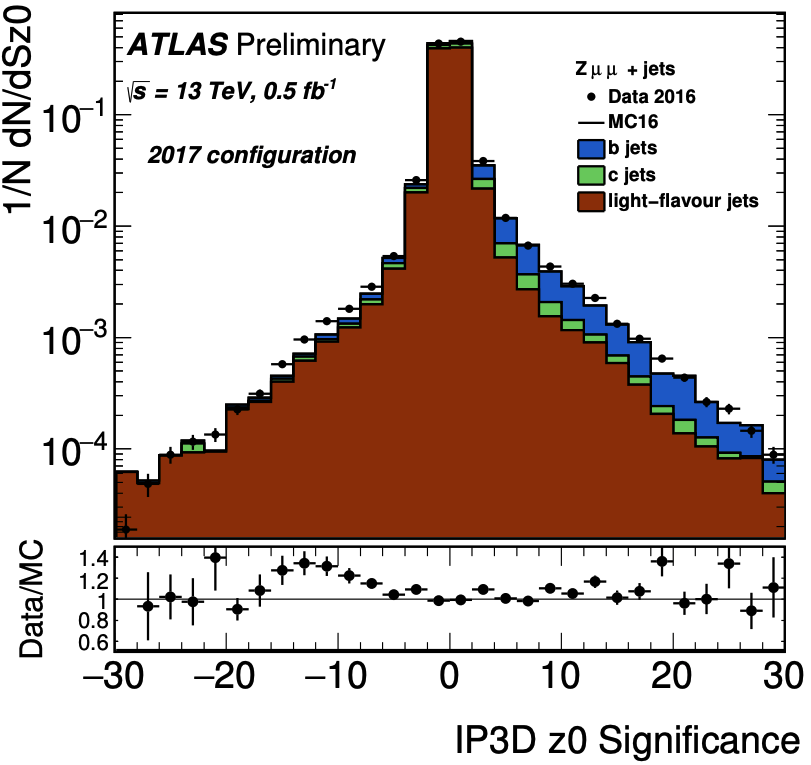
\includegraphics[width=0.48\linewidth]{figures/objects/IP3D_z0}}

  \caption{Data-Monte Carlo comparisons of the
transverse ($d_{0}$) and longitudinal ($z_{0}$) impact parameter significance
values for IP3D selected charged tracks in the leading jet of a $Z\to\mu\mu +
\text{jets}$ dominated sample \cite{Chisholm:bjet}.}
  \label{sec:objects:impact_parameters}
\end{figure}

In 2017 two new tools were included into the tagger
\cite{ATL-PHYS-PUB-2017-013}; a Recurrent Neural Network (RNN) impact parameter
tagger (RNNIP) and a Soft Muon Tagger (SMT).  The RNNIP
\cite{ATL-PHYS-PUB-2017-003} exploits the fact that $b$-jets tend to have many
tracks with highly significant impact parameters, while $l$-jets do not, as
seen in \Cref{sec:objects:RNNIP}.  The SMT \cite{Sciandra:2287545} searches for
muons coming from the semi-leptonic decays of $b$-hadrons and $c$-hadrons to
discriminate against $l$-jets which have much softer muons or none at all. The
separation power of the SMT is shown in \Cref{sec:objects:SMT}.

\begin{figure}[!htbp]
  \centering
  \subcaptionbox{$b$-jets}{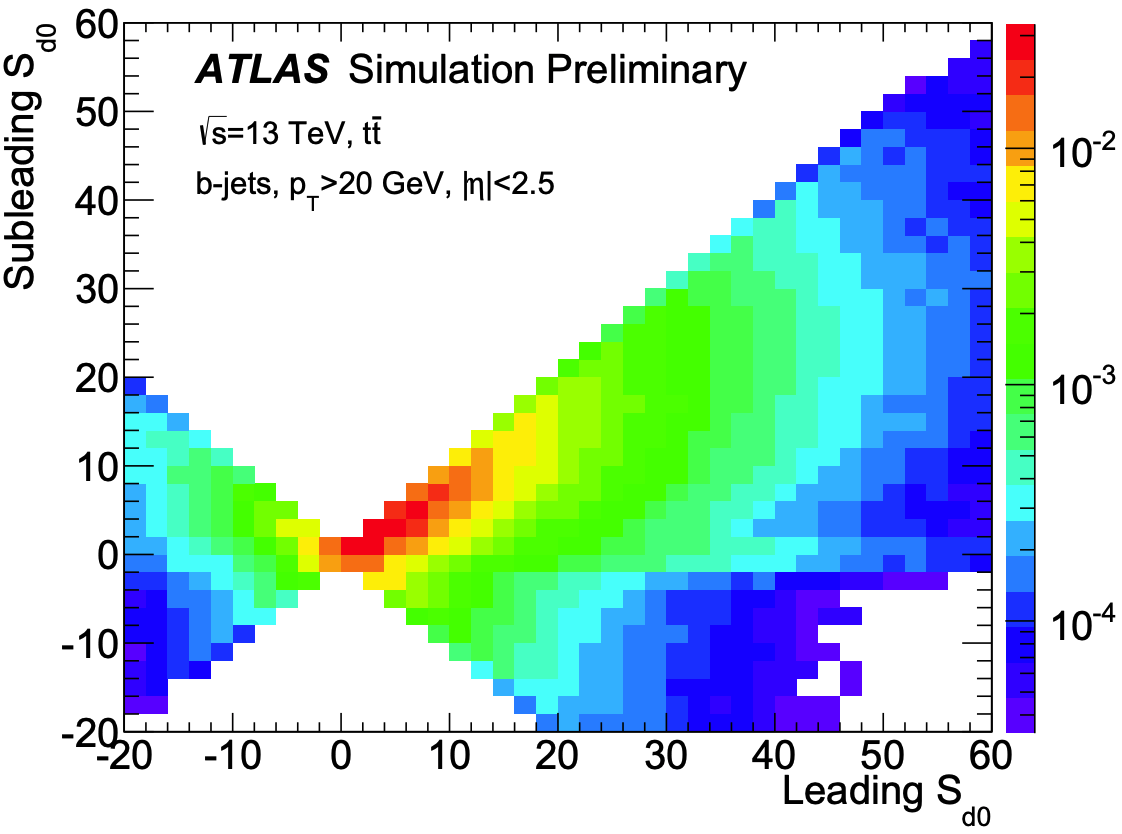
\includegraphics[width=0.48\linewidth]{figures/objects/RNNIP_b_jets}} \hfill
  \subcaptionbox{$l$-jets}{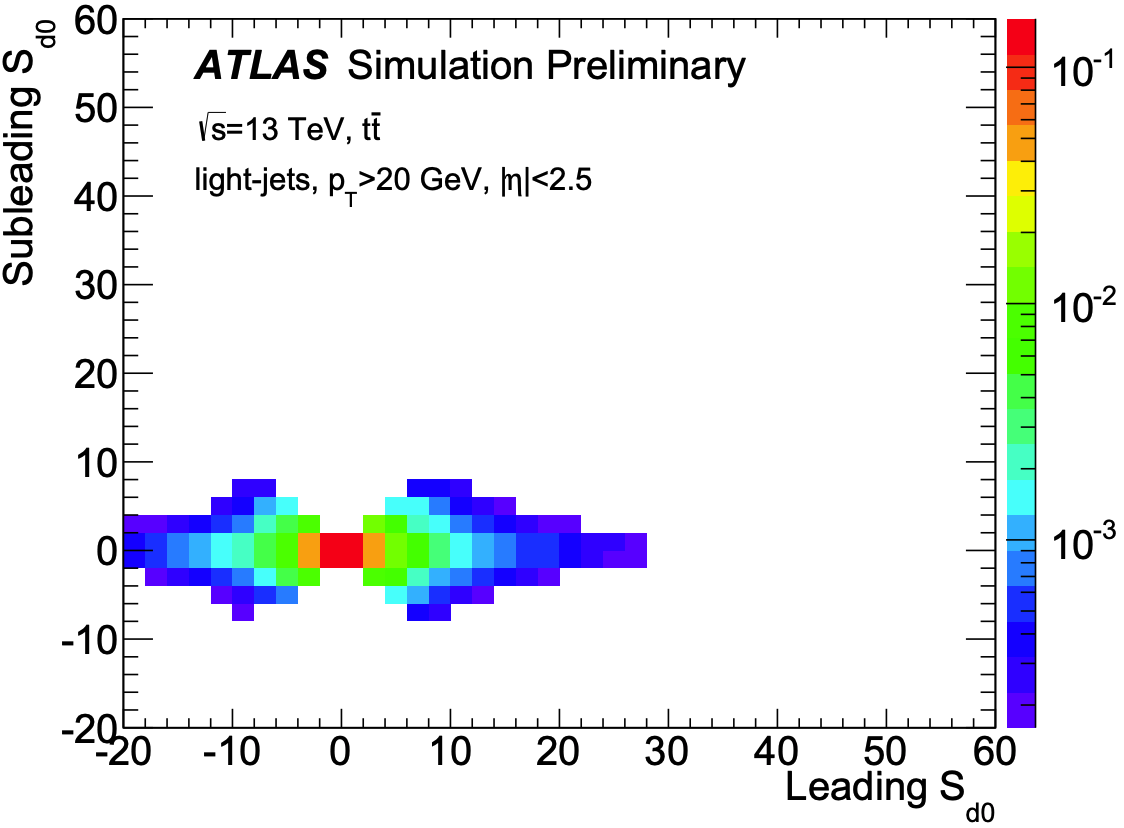
\includegraphics[width=0.48\linewidth]{figures/objects/RNNIP_l_jets}}

  \caption{The distribution of the transverse impact parameter significance $S_{d0}$ for the leading $d_{0}$ significance track and subleading $d_{0}$ significance track for $b$-jets (left) and $l$-jets (right) \cite{Chisholm:bjet}.}
  \label{sec:objects:RNNIP}
\end{figure}

\begin{figure}[!htbp]
  \centering
  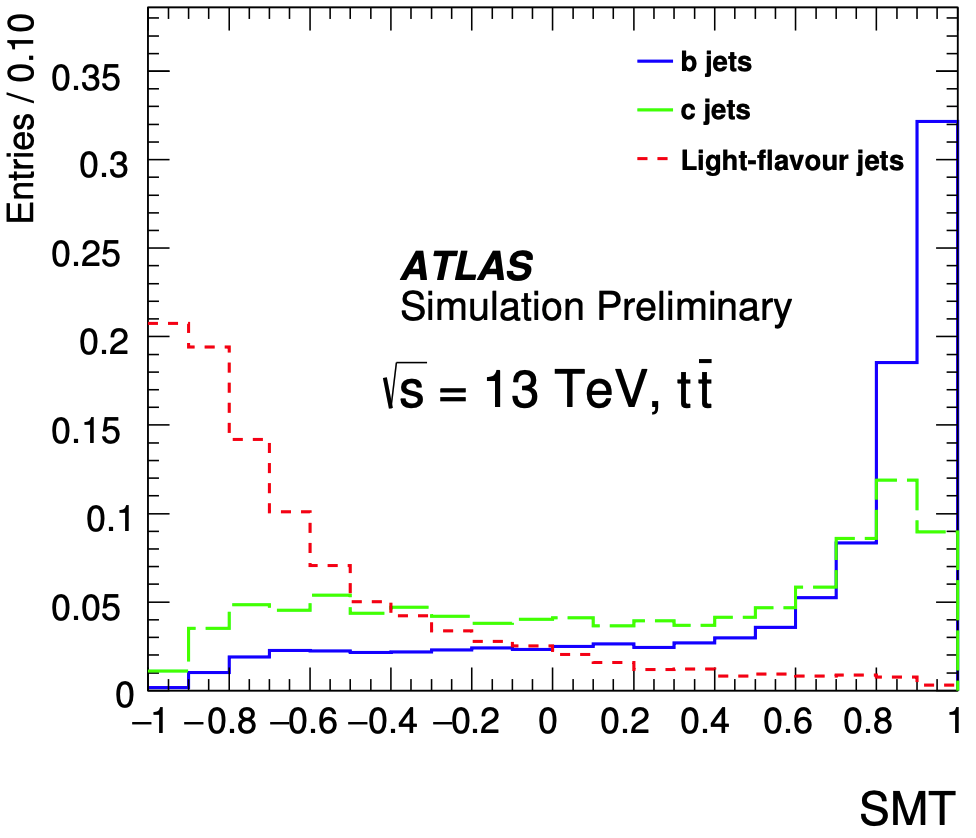
\includegraphics[width=0.5\linewidth]{figures/objects/SMT}
  \caption{Normalized BDT response in simulated $t\bar{t}$ events of the SMT for reconstructed muons associated to $b$-jets (blue), $c$-jets, (green) and light-flavour jets (red) \cite{Chisholm:bjet}.}
  \label{sec:objects:SMT}
\end{figure}

All of the above algorithms' outputs, along with jet kinematic information, are
used as input to the \texttt{MV2c10} algorithm as seen in
\Cref{sec:objects:BDT_flowchart}.  The output is a discriminant score which
indicates how $b$-jet-like or how un-$b$-jet-like the jet in question is,
compared to the training sample used, as shown in
\Cref{sec:objects:MV2c10_output}.  The performance is calibrated in data using
jets containing a muon, indicating the semileptonic decay of the $b$-hadron,
and a correction is derived for the simulated events \cite{Aaboud:2018xwy}.

\begin{figure}[!htbp]
  \centering
  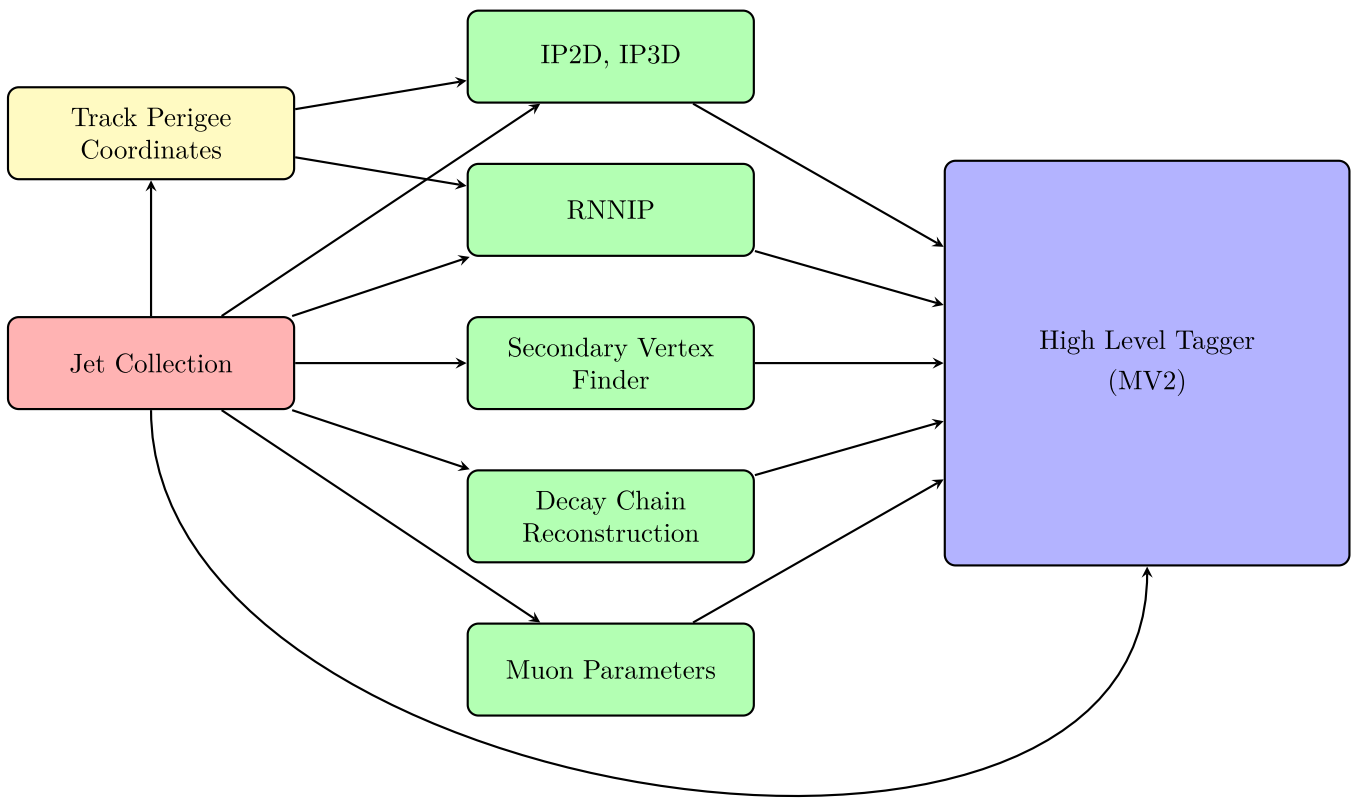
\includegraphics[width=0.8\linewidth]{figures/objects/BDT_flowchart}
  \caption{Flowchart of inputs to the \texttt{MV2c10} $b$-tagging algorithm \cite{Feickert:2690521}.}
  \label{sec:objects:BDT_flowchart}
\end{figure}

\begin{figure}[!htbp]
  \centering
  \subcaptionbox{\texttt{MV2c10} discriminant for $b$-jets compared to $c$-jets and $l$-jets in simulated $t\bar{t}$ events.}{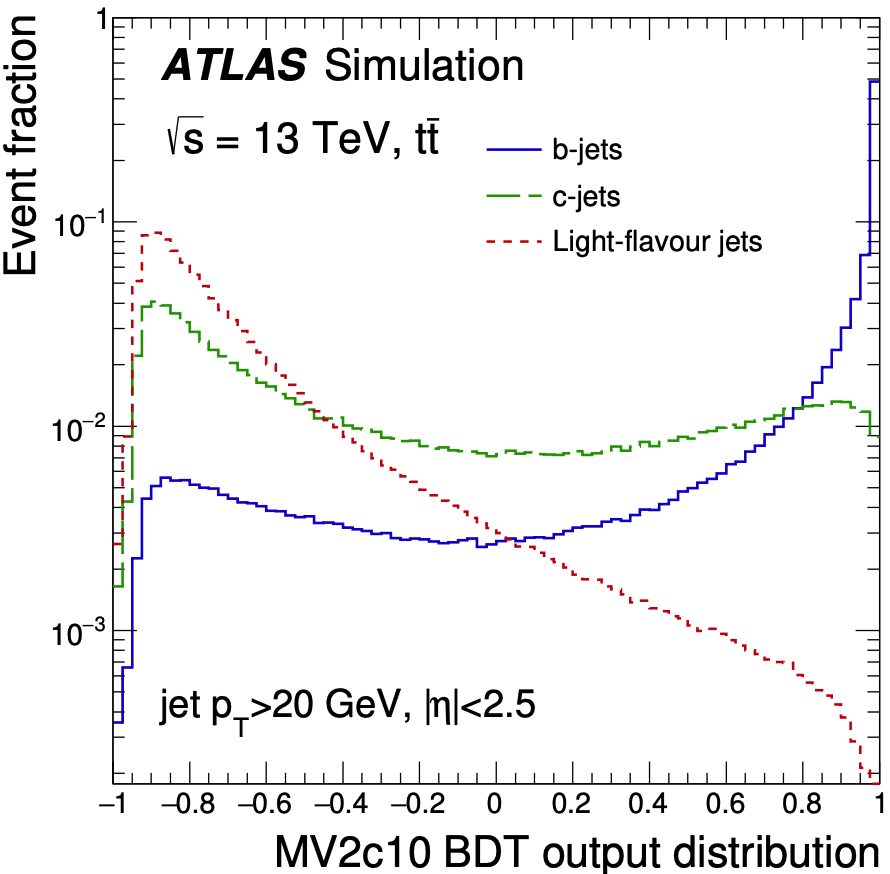
\includegraphics[width=0.48\linewidth]{figures/objects/BDT_output}} \hfill
  \subcaptionbox{$l$-jet and $c$-jet rejection factors as a function of $b$-jet tagging efficiency of the \texttt{MV2c10} BDT.}{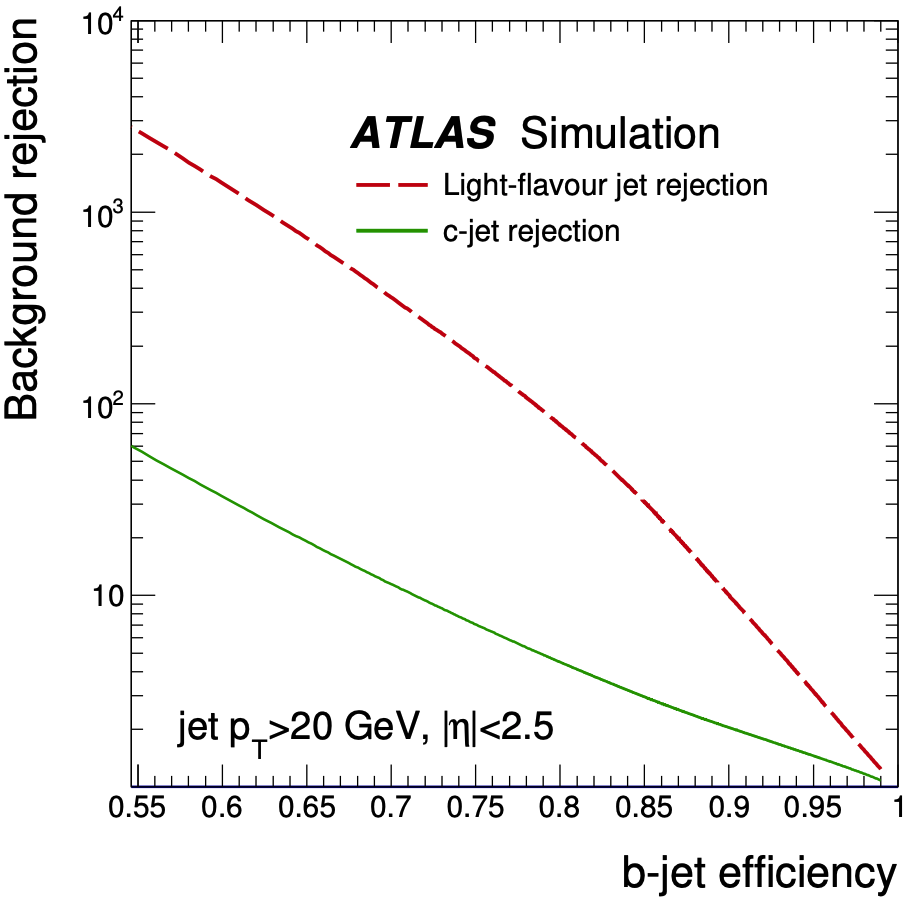
\includegraphics[width=0.48\linewidth]{figures/objects/b_jet_efficiency}}

  \caption{Performance of the \texttt{MV2c10} BDT for
the 2016 optimization in simulated $t\bar{t}$ events.  The performance was
evaluated on $t\bar{t}$ events simulated using \textsc{Powheg} interfaced to
\textsc{Pythia6} \cite{Aaboud:2018xwy}.}
  \label{sec:objects:MV2c10_output}
\end{figure}
